%avoid page number on blank pages when cleared
\thispagestyle{empty}
\cleardoublepage
\chapter{Experiments and Results}
\label{chap:experiments}

%Introduce Chapter: 3 experiments (test set size = 3) to test the whole
%shape matching methodology. Its separated in three main processes: initial
%processing, automatic shape matching and manual fixing. The results are 
%presented and discussed.

In this chapter the different experiments carried out to test the performance
of the shape matching solution are 
presented, explaining the reason for their choice and the test objectives.
Then the results are presented and discussed, pointing out the advantages and drawbacks of the suggested
shape matching model that are inferred from the first ones.

\section{Experiments}
\label{sec:experiments}

In order to test the implemented solution, three digital images of worms in liquid
media were provided by Johan Henriksson at the \emph{Department of Bioscience and Nutrition, Karolinska Institutet}.
Each image corresponds to a different difficulty level, 
following the criteria of number of worms and degree of overlap. Thus the greater the number 
of worms in the image and the greater the number of worms that are connected by overlapping,
the greater the difficulty level. The overlapping degree is determined by the number
of worms that belong to the different \emph{worm clusters} (first defined in Sec. \ref{sec:reasoning})
and the number of \emph{worm clusters} in the image.
The selected images are named \emph{test image 1}, \emph{test image 2} and \emph{test image 3}
and are displayed in an increasing difficulty level order, from the easiest to the hardest. 
The characteristics of the test set are presented in table \ref{tab:testset}.


\begin{table}[h]
  \caption{Test set images characteristics}
\begin{center}
\begin{tabular}[h]{|>{\columncolor[gray]{0.9}} p{2cm} |p{3cm} | p{2.8cm} | p{3cm}| p{2.8cm} |}
    \hline
    \rowcolor[gray]{.9}
    Test Image & Number of Isolated Worms & Number of Worm Clusters & Number of Worms per Clusters  & Total Number of Worms\\
    \hline
    Test 1 & 11/19 (57.8\%) & 3 & 8/19 (42.1\%) & 19 \\
    \hline
    Test 2 & 8/33 (24.2\%) & 3 & 25/33 (75.7\%)& 33 \\    
    \hline
    Test 3 & 13/38 (34.2\%)& 5 & 25/38 (65.7\%) & 38 \\
    \hline 
  \end{tabular}
\end{center}
  \label{tab:testset}
\end{table}


For each test image a series of experiments were carried out to test the performance of
the different processes that are involved in the solution methodology. The entire 
shape fitting process was divided into three stages that represent the 
main fitting steps. These are: \emph{Initial Processing}, \emph{Automatic Shape Matching} and
\emph{Matching Manual Fixing}.\\

The \emph{Initial Processing} involves all the image processing steps that are performed 
before the shape matching optimization process, as explained in Sec.\ref{sec:solmet},
such as: thresholding, distance transformation, skeletonization, 
clustering, endpoint detection and worm profiling. Among these, the distance transformation
and skeletonization follow already implemented and tested algorithms (covered in Sec.\ref{sec:metdt}
and Sec.\ref{sec:metsk}) and produce straight-forward results, so there is no need to further analyse them.
The clustering process follows the skeletonization process and is straight-forward as well.
On the other hand the thresholding, endpoint detection and worm profiling processes vary 
from image to image, so different experiments are carried out in order to test these subprocesses
for the test set.\\

The \emph{Automatic Shape Matching} stage consists of experiments dealing with the automatic
optimization process to match \emph{worm clusters} and contour-following technique to match 
\emph{isolated worms} that produce the initial fitting of the worms. These 
experiments attempt to measure the efficacy and time efficiency of different variations of the
matching algorithm, in order to make a conclusion about properties of the algorithm and the feasibility 
of the automatic solution.\\
The third stage, \emph{Matching Manual Fixing}, attempts to measure the type and number of 
manual adjustments that must be performed by the user in order to correct the 
wrongly assigned automatic matchings. The experiment is also 
aimed at determining how much the efficacy of the automatic solution can be improved, in
order to get a better matching. Once the best possible matching is found through manual fixing,
the stability of the best match is studied by comparing the energy to the second and third best
matches.\\

The experiments were executed on a personal computer with a 2.00 GHz AMD Turion 
Dual-Core Mobile Processor, 1 MB Microprocessor cache and 3Gb of RAM Memory, 
on Linux Operating System, Ubuntu Distribution.

\section{Results}
\label{sec:results}

In this section the results obtained for the test set are presented and discussed.
The results are distributed in the three main stages: \emph{Initial Processing}, \emph{Automatic Shape Matching} and
\emph{Matching Manual Fixing}. In the section \emph{Initial Processing} the results for the three different 
images in the test set are presented. On the other hand the section \emph{Shape fitting} presents the different
results for the stages \emph{Automatic Shape Matching} and \emph{Matching Manual Fixing} for every test image
individually.

\subsection{Initial Processing}
\label{sec:initproc}

This section presents the results for the experiments carried out over the test set for the 
processes: thresholding and endpoint finding. Then a brief discussion about
the result for the worm profiling process is also presented.

\subsubsection*{Thresholding}

As explained in Sec.\ref{sec:thresimp} \emph{Endrov} has implementations for the 
thresholding filters \emph{Fukunaga}, \emph{Max entropy}, \emph{Otsu} and \emph{Percentile}.
In order to select an appropriate thresholding
filter, the four previously mentioned were tried on every test image, tweaking the
input parameters until the best possible binary image was obtained from every one.
From visual inspection, the \emph{Percentile} filter generated the
best binary images for the three tests. 
The best percentile values for every test image are shown in table \ref{tab:threshold}.
The second closest method was \emph{Fukunaga}
that produced acceptable solutions after the combination of binary images
generated from different number of classes, however the results were not as good as
the ones obtained with \emph{Percentile} and also required more processing.

\begin{table}[h]
  \caption{Best percentile values for Percentile Thresholding of test images}
\begin{center}
\begin{tabular}[h]{|>{\columncolor[gray]{0.9}} c |c|c|c|}
    \rowcolor[gray]{.9}
    \hline
    Test & Test Image 1 & Test Image 2 & Test Image 3\\
    \hline
    Percentile Value & 0.074 & 0.1 & 0.11\\
    \hline
  \end{tabular}
\end{center}
  \label{tab:threshold}
\end{table}

The resultant best percentile values oscillate between $0.074$ and $0.11$, and are 
simple to determine using \emph{Endrov}.   

\subsubsection*{Endpoint detection}

This section presents the results for the detection of worm endpoints.
Table \ref{table:endtable} shows the number of worm endpoints that are
automatically detected and those that have to be manually added in order
to cover all the endpoints for the worms in the image.

\begin{table}[h]
  \caption{Worm endpoints detection and fixing for the test set}
\begin{center}
\begin{tabular}[h]{|>{\columncolor[gray]{0.9}} p{2cm} |p{1.9cm}|p{2cm}|p{2.2cm}|}
    \rowcolor[gray]{.9}
    \hline
    Test Image & Total Endpoints & Detected Endpoints & Manually Added Endpoints\\
    \hline
    Image 1 & 38 & 38 (100\%) & 0 \\
    \hline 
    Image 2 & 66 & 53 (80\%) & 13 \\
    \hline 
    Image 3 & 76 & 57 (75\%) & 19 \\
    \hline
  \end{tabular}
\end{center}
  \label{table:endtable}
\end{table}

Table \ref{table:endtable} presents the number of endpoints identified
automatically for every test image and the number of endpoints that must be added manually.
It shows that a large number of worms belonging
to \emph{worm clusters} increases the probability to have endpoints overlapping, 
as does a high density of worms.
Considering the large number of worms that belong to worm clusters 
for images two and three (as show in  Table \ref{tab:testset}) and the low
number of clusters for each one (which increases the overlapping), the amount
of missing endpoints can be considered fairly low and it is feasible to add them manually.

\subsubsection*{Worm Profiling}

In order to generate an accurate worm profile of the worms present in the image
it is necessary to have \emph{isolated worms} in the processed image. The percentage 
of \emph{isolated worms} for every image were $57.8\%$, $24.2\%$ and $34.2\%$ 
respectively,
oscillating between $8$ and $13$ worms, as shown in Table \ref{tab:testset}. 
For all images, the generated worm profiles were sufficiently accurate to
conduct the optimization shape matching process, whose results are presented in 
the subsections named \emph{Automatic Shape Matching} for every test image result.

\subsection{Shape Matching}

In this section the results for the second and third stage in the 
solution methodology are presented, as described above in Sec. \ref{sec:experiments}, which consist
in \emph{Automatic Shape Matching} and \emph{Matching Manual Adjustment}. 
For the \emph{Automatic Shape Matching} subsection the results for a series of four 
variations of the matching algorithm are presented, focusing on the matching accuracy 
and time performance. The two main variants are: Path Guessing and Every Path. 
Path Guessing is the version of the algorithm in which every guessed path is favored
by an improvement in its shape optimization value, by reducing it to the half. So when 
a conformation is to be chosen for an endpoint the value of the guessed path is more likely
to be selected. On the other hand, the Every Path variant considers every possible conformation for every endpoint.
Each variant is executed with and without manually adding the missing endpoints.\\

The \emph{Matching Manual Fixing} presents the results of modifying the erroneous matches
obtained by the best automatic matching algorithm, showing the resulting best
possible matching image and indicating the number of worm shapes that had to be 
re-arranged. This process is done manually: The user detects the wrong matching visually 
and selects two endpoints to obtain the best optimized shape that connects them, as
explained in Sec. \ref{sec:matchfix}. An operation (as used in the tables for this section) 
is considered to be the process of selecting two endpoints and generate a new shape.\\

Then a subsection \emph{Matching Energy} is presented in which the distribution of
the energy values for the different conformations is discussed. This section presents
a graph showing the different energy values (objective function) for the correct conformation
and the next two best conformations for every endpoint (of those having three or more conformations). 
The correct conformation corresponds to the one that is constructed between the two endpoints that
belong to the worm in the image. The other two are conformations that start in the
selected endpoint and end in a wrong one.


\subsubsection*{Automatic Shape Matching (Test Image 1)}

Since for the test image 1 all the endpoints are found automatically, as shown in 
Table \ref{table:auto1}, the results presented here show the matching efficiency and
runtime just for the variations Every Path and Path Guessing, that include all the
worm endpoints. Table \ref{table:auto1} presents the obtained results.

\begin{table}[h!]
  \caption{Results of automatic worm shape matching on test image 1}
  \begin{center}
  \begin{tabular}{|>{\columncolor[gray]{0.9}} p{3cm}|p{2.8cm}|p{2.8cm}|p{2.8cm}|c|}
    \hline
    \rowcolor[gray]{.9}
    Path finding & Isolated Worms matching & Cluster Worms matching 
    & Total Matching 
    & Time (s) \\ 
    \hline
    Every Path & 11/11 (100\%) & 6/8 (75\%) & 17/19 (89.5\%)& 6.47 \\
    \hline
    P.Guessing & 11/11 (100\%) & 8/8 (100\%) & 19/19 (100\%) & 7.53 \\
    \hline
  \end{tabular}
\end{center}
  \label{table:auto1}
\end{table}

It can be observed that in both variations of the algorithm the 
\emph{isolated worms} were all matched. For the Every Path variation 
three quarters of the worms in clusters were matched correctly.
On the other hand the Path Guessing variation managed to match automatically 
all the worms in the image. The execution time is slightly higher for the
Path Guessing Variation, as expected because of the extra calculations that
must be performed to calculate the best paths departing from each endpoint.\\

For this image, the Path Guessing variant represented an improvement in 
the solution, by inducing the shape produced from guessed paths to be more
likely to be selected. On the other hand, at first glance, the isolated
worms seem to be matched regardless of the algorithm variant, as expected.\\
The best matching for test image 1, corresponding to the Path Guessing variation, is shown in Fig.\ref{fig:best1}.


\begin{figure}[h!]
  \centering
  \subfloat[Best Match]{\label{best1}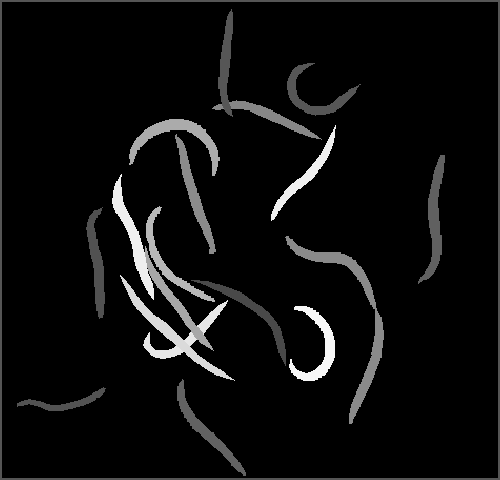
\includegraphics[scale=0.34]{results/test1/complete-frame1}}
\qquad
  \subfloat[Best Match over original image]{\label{bestbg1}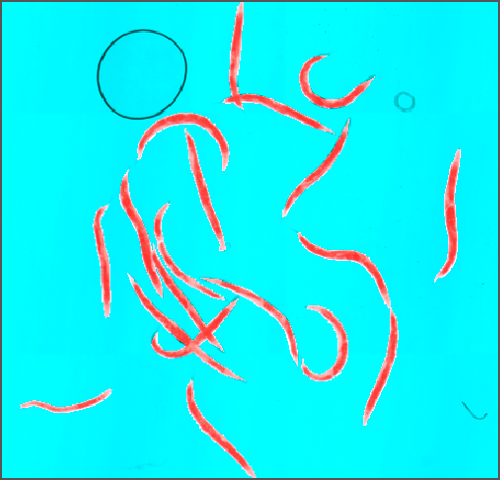
\includegraphics[scale=0.34]{results/test1/complete-framebg1}}
  \caption{Best automatic shape matching on test image 1}
  \label{fig:best1}
\end{figure}


\subsubsection*{Automatic Shape Matching (Test Image 2)}

The results for automatic matching on test image 2 are shown in table \ref{tab:tab2}.

\begin{table}[h]\begin{tabular}{|>{\columncolor[gray]{0.9}} p{3cm}|p{2.8cm}|p{2.8cm}|p{2.8cm}|c|}
    \hline
    \rowcolor[gray]{.9}
    Path finding & Isolated Worms matching & Cluster Worms matching 
    & Total Matching 
    & Time (s) \\ 
    \hline  
    Every Path - me & 8/8 (100\%) & 7/25 (28\%) & 15/33 (45.4\%) & 21.8 \\ 
    \hline
    P.Guessing - me & 8/8 (100\%) & 10/25 (40\%) & 18/33 (54.5\%) & 23.7\\
    \hline
    Every Path + me & 8/8 (100\%)& 15/23 (65.2\%) & 23/33 (69.7\%)& 42.3 \\
    \hline
    P.Guessing + me & 8/8 (100\%)& 21/25 (84\%) & 29/33 (87.8\%) & 45 \\
    \hline
  \end{tabular}
  \label{tab:tab2}
  \caption{Results of automatic worm shape matching on test image 2, without and with missing endpoints (me)}
\end{table}

It can be observed that for every variation the Isolated Worms were matched
totally. For the two variations that have missing endpoints just around
the half of the total worms could be matched. Though the execution time is
slower, which is expected given the decrease of feasible paths, not having an
endpoint of a worm makes impossible to find a shape that matches it correctly.
For the variations that include endpoints the results are considerably better.
It can be observed that the Path Guessing variation
increases the matching accuracy, in both missing and not missing
endpoints set of variations. The execution time also increases
when all endpoints are added, as expected. 
For the Path Guessing variation the matching percentage increases considerably,
although is slightly slower than Every Path.
In the best case the automatic matching solution manages to fit the shape
for all the isolated worms and a high percentage of the clustered worms in
less than a minute.

\subsubsection*{Matching Manual Adjustment (Test Image 2)}

Path Guessing with no missing endpoints gave the best result,
with just $4$ worms wrongly matched among $33$. Fig.\ref{fig:best2} shows the matchings.

\begin{figure}[h]
  \centering
  \subfloat[Best Automatic Match]{\label{test2:best2}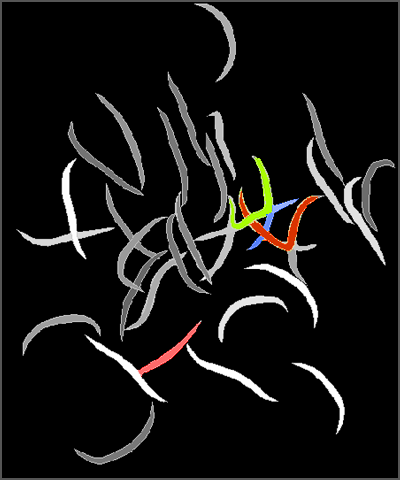
\includegraphics[scale=0.45]{results/test2/guessing-nobgframe}}
\qquad
  \subfloat[Best Automatic Match over original image]{\label{bestbg1}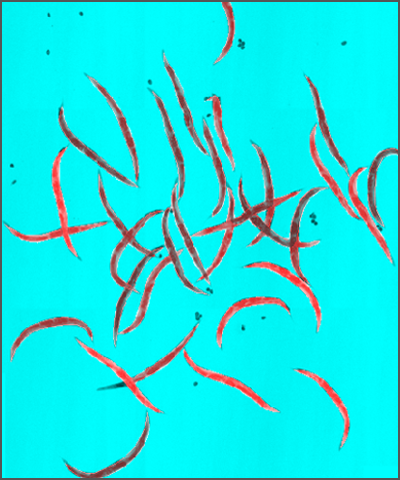
\includegraphics[scale=0.45]{results/test2/guessing-bgframe}}
\qquad
  \subfloat[Manually Adjusted Match]{\label{test2:bestbg2}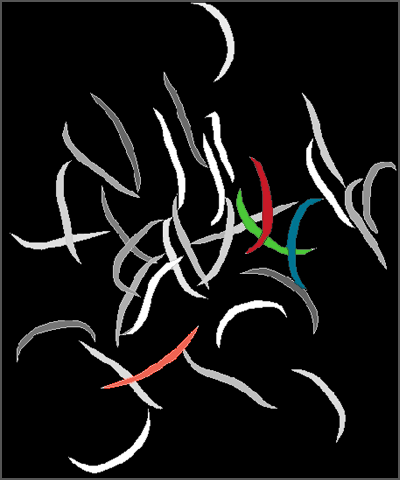
\includegraphics[scale=0.45]{results/test2/frame2-allnobg}}
\qquad
  \subfloat[Manually Adjusted Match over original image]{\label{bestbg1}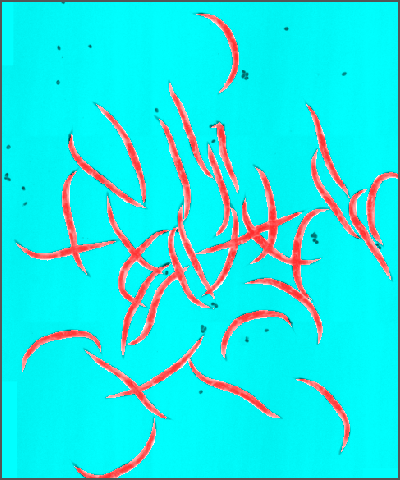
\includegraphics[scale=0.45]{results/test2/frame2-all}}

\caption{Best automatic shape matching and Manual match fixing on test image 2. Colored shapes and outlines in images
    \ref{test2:best2} and \ref{test2:bestbg2} indicate incorrectly detected worms}
\label{fig:best2}
\end{figure}

Manual adjustment required selecting two endpoints that correspond to an actual worm shape. After selecting the
endpoints the assigned shapes starting at this endpoints are removed
and the best shape that connects the two selected endpoints is added.
Finally all of the worms in the image could be fitted.


\subsubsection*{Automatic Shape Matching (Test Image 3)}

The results for automatic matching on test image
3 are presented in table \ref{tab:tab3}. The four variations for the algorithm are shown.

\begin{table}[h!]\begin{tabular}{|>{\columncolor[gray]{0.9}} p{3cm}|p{2.8cm}|p{2.8cm}|p{2.8cm}|c|}
    \hline
    \rowcolor[gray]{.9}
    Path finding & Isolated Worms matching & Cluster Worms matching 
    & Total Matching 
    & Time (s) \\ 
    \hline  
    Every Path - me & 13/13 (100\%) & 5/25 (20\%) & 18/38 (47.3\%) & 26.4 \\ 
    \hline
    P.Guessing - me & 13/13 (100\%) & 7/25 (28\%) & 20/38 (52.6\%) & 28.7\\
    \hline
    Every Path + me & 13/13 (100\%)& 13/25 (52\%) & 26/38 (68.4\%)& 36.2 \\
    \hline
    P.Guessing + me & 13/13 (100\%)& 16/25 (64\%) & 29/38 (76.3\%) & 39.8 \\
    \hline
  \end{tabular}
  \label{tab:tab3}
  \caption{Results of automatic worm shape matching on test image, without and with missing endpoints (me)}
\end{table}

The isolated worms were always matched successfully.
Every Path and Path Guessing with missing points, 
the total matching is around the half of the total. 
With missing endpoints adjusted, the level of accuracy increases considerably.
Calculation is slower with more endpoints.
The Path Guessing variations is always better than Every Path, and is slightly slower.\\
The best variation was the Path Guessing with no missing endpoints, managing
to match all the \emph{isolated worms} and a total of three quarters of the 
whole image.

\subsubsection*{Matching Manual Adjustment (Test Image 3)}

The Path Guessing without missing endpoints turned out to be the best one, with $9$ worms wrongly matched among $38$.
Fig.\ref{fig:best3} presents four images for this algorithm.

\begin{figure}[h!]
  \centering
  \subfloat[Best Automatic Match]{\label{test3:best3}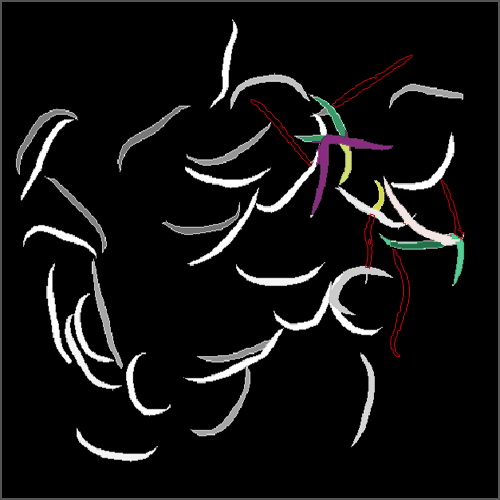
\includegraphics[scale=0.35]{results/test3/guess-nobg}}
\qquad
  \subfloat[Best Automatic Match over original image]{\label{bestbg1}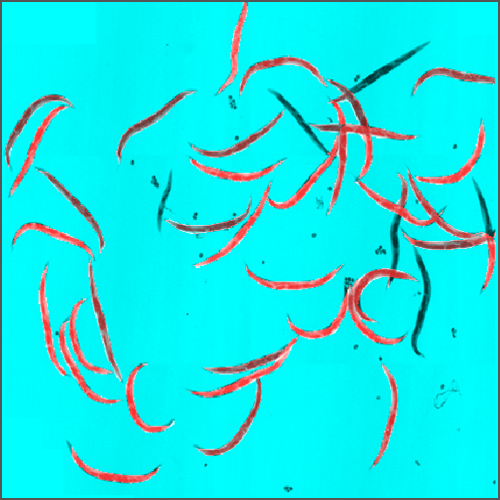
\includegraphics[scale=0.35]{results/test3/guess-bg}}
\qquad
  \subfloat[Manually Adjusted Match]{\label{test3:bestbg3}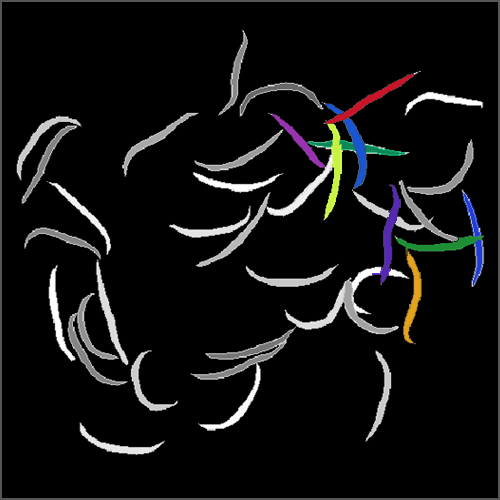
\includegraphics[scale=0.35]{results/test3/all-nobg}}
  \label{best3:c}
\qquad
  \subfloat[Manually Adjusted Match over original image]{\label{bestbg1}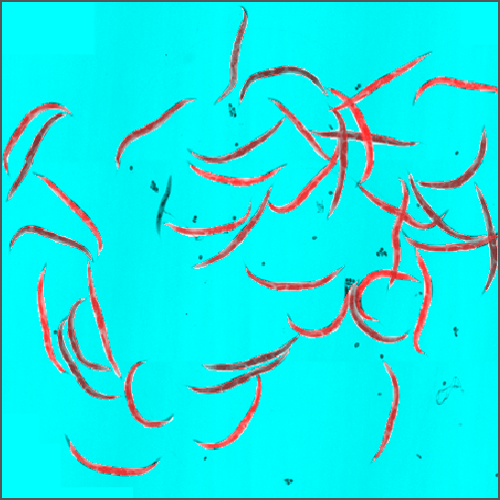
\includegraphics[scale=0.35]{results/test3/all-bg}}
  \caption{Best automatic shape matching and Manual match fixing on test image 3. Colored shapes and outlines in images
    \ref{test3:best3} and \ref{test3:bestbg3} indicate incorrectly detected worms}
  \label{fig:best3}
\end{figure}


Nine operations were required to manually adjust the incorrectly matched worms.
All the worms in the image could then be matched and fitted.

\subsection{Matching Energy}

The energy for the best three conformations in each endpoint is shown in Fig.\ref{fig:energy123}.
The first is correct and matches the worm, the other two match wrong endpoints.\\
Recall that the energy function, covered
in Sec.\ref{sec:clusterfit}, evaluates the distance between a matching shape
and a matched shape as the percentage of background pixels contained in the 
area covered by the matching shape, so all the possible energy values are
contained in the interval $[0,1]$ and the optimized shapes tend to take values
from one to three decimals close to $0$.

\captionsetup[subfloat]{farskip=-0.8cm,captionskip=-0.2cm}

%Distance between images could be reduced to make graphs larger
\begin{figure}[htp]
  \begin{center}
    \subfloat[Image 1]{\label{fig:energy1b}\includegraphics[scale=0.54]{results/test1/energy-graph}}\\
    \subfloat[Image 2]{\label{fig:energy2b}\includegraphics[scale=0.54]{results/test2/energy-graph}}\\
    \subfloat[Image 3]{\label{fig:energy3b}\includegraphics[scale=0.54]{results/test3/energy-graph}}
  \end{center}
  \caption{Energy value for the best three conformations by endpoint ID on test
images. The right conformation is red. The selected endpoints correspond to worms in worm clusters that
have more than two possible conformations.}
  \label{fig:energy123}
\end{figure}
\showcaptionsetup{subfloat}

\subsubsection*{Test Image 1}

For most endpoints the correct conformation has the lowest energy value.
In two cases a wrong conformation had a lower energy value than the correct
one. The third best conformation always has higher energy than the correct conformation.\\

\subsubsection*{Test Image 2}


It can be observed that the second best conformation (in green) is in all 
the cases worst that the best conformation, normally from two to four times 
in terms of the energy function value, thus the correct conformation is 
either the best or the second best conformation, from all the possible.
In this case only four endpoints among twenty nine show a better energy
function value for the best next conformation (in red) over the correct 
conformation (in blue). This coincides directly with the results shown
in Table \ref{tab:tab3} where, for the best automatic solution (Path Guessing),
the amount of worms successfully matched was 29/33, which is only four worms
away from the optimal solution, the same number of endpoints in which the
correct conformation is not the best in value. In fact, the difference of 
values between the correct and best next conformation for the these four
endpoints is close enough to think that a more sensitive objective function
could retrieve the correct conformation for all the cases for the automatic
algorithm.\\ 

\subsubsection*{Test Image 3}

Among the 22 endpoints, for 9
of them the second best conformation resulted to have a better energy value
than the correct conformation. This is consistent with the results presented
in Table \ref{tab:tab3} where for the best variation (Path Guessing), the
number of wrongly detected worms is also nine. This means that an incorrect 
path is considered to be more likely to be a worm starting from this
endpoints. For every endpoint, with the exception of one, the second best 
solution is worse than the correct solution. So the energy value of the 
correct solution is either the best or the second best.\\

Given that for this image the amount of worms that belong to clusters
is high (25), the number of possible paths starting
from every endpoint is high and so is the number of wrong conformations.
Since so many correct conformations did not have the lowest energy value,
the energy formulation must not be sensitive enough. However
the differences between the correct and selected conformations for
these cases are close (just as for test image 2), so a more sophisticated objective function could lead
to better results.\\



